\section{Pruning Neurons to Shrink Neural Networks}\label{sec2}
As discussed in Section \ref{sec1} our aim is to leverage the highly non-uniform distribution of the learning representation in pre-trained neural networks to eliminate redundant neurons, without focusing on individual weight parameters. Taking this approach enables us to remove all the weights (incoming and outgoing) associated with a non-contributing neuron at once. We would like to note here that in an ideal scenario, based on the neuron interdependency theory put forward by \cite{mozer1989skeletonization}, one would evaluate all possible combinations of neurons to remove (one at a time, two at a time, three at a time and so forth) to find the optimal subset of neurons to keep. This is computationally unacceptable, and so we will only focus on removing one neuron at a time and explore more ``greedy'' algorithms to do this in a more efficient manner.

The general approach taken to prune an optimally trained neural network here is to create a ranked list of all the neurons in the network based off of one of the 3 proposed ranking criteria: a brute force approximation, a linear approximation and a quadratic approximation of the neuron's impact on the output of the network. We then test the effects of removing neurons on the accuracy and error of the network. All the algorithms and methods presented here are easily parallelizable as well.

One last thing to note here before moving forward is that the methods discussed in this section involve some non-trivial derivations which are beyond the scope of this paper. We are more focused on analyzing the implications of these methods on our understanding of neural network learning representations. However, a complete step-by-step derivation and proof of all the results presented is provided in the Supplementary Material as an Appendix.

\subsection{Brute Force Removal Approach}
This is perhaps the most naive yet the most accurate method for pruning the network. It is also the slowest and hence possibly unusable on large-scale neural networks with thousands of neurons. This method explicitly evaluates each neuron in the network. The idea is to manually check the effect of every single neuron on the output. This is done by running a forward propagation on the validation set $K$ times (where $K$ is the total number of neurons in the network), turning off exactly one neuron each time (keeping all other neurons active) and noting down the change in error. Turning a neuron off can be achieved by simply setting its output to 0. This results in all the outgoing weights from that neuron being turned off. This change in error is then used to generate the ranked list. 

\subsection{Taylor Series Representation of Error}
Let us denote the total error from the optimally trained neural network for any given validation dataset by $E$. $E$ can be seen as a function of $O$, where $O$ is the output of any general neuron in the network. This error can be approximated at a particular neuron's output (say $O_k$) by using the 2nd order Taylor Series as,

\begin{align}
\hat E(O) \approx E(O_k) + (O-O_k)\cdot \left.\pdv{E}{O}\right|_{O_k} +  0.5\cdot (O-O_k)^2\cdot \left.\pdv[2]{E}{O}\right|_{O_k}\label{eq:ts1},
\end{align}


When a neuron is pruned, its output $O$ becomes 0. %From equation \ref{eq:ts1}, the contribution $E(0)$ of this neuron, then becomes:

%\begin{align}
%\hat E(0) \approx E(O_k) - O_k\cdot \left.\pdv{E}{O}\right|_{O_k} +  0.5\cdot O_k^2\cdot \left.\pdv[2]{E}{O}\right|_{O_k}\label{eq:ts2}
%\end{align}

Replacing $O$ by $O_k$ in equation \ref{eq:ts1} shows us that the error is approximated perfectly by equation \ref{eq:ts1} at $O_k$. So:%Using this and equation \ref{eq:ts2} we get:

\begin{align}
\Delta E_k = \hat E(0) - \hat E(O_k)= - O_k\cdot \left.\pdv{E}{O}\right|_{O_k} + 0.5\cdot O_k^2\cdot \left.\pdv[2]{E}{O}\right|_{O_k}\label{eq:ts3},
\end{align}

where $\Delta E_k$ is the change in the total error of the network when exactly one neuron ($k$) is turned off. Most of the terms in this equation are fairly easy to compute, as we have $O_k$ already from the activations of the hidden units and we already compute $\pdv{E}{O}|_{O_k}$ for each training instance during backpropagation. The $\small{\pdv[2]{E}{O}|_{O_k}}$ terms are a little more difficult to compute. This is derived in the appendix and summarized in the sections below. 



\subsubsection{Linear Approximation Approach}
We can use equation \ref{eq:ts3} to get the linear error approximation of the change in error due to the $k$th neuron being turned off and represent it as $\Delta E_{k}^1$ as follows:

\begin{align}
\Delta E_{k}^1 = - O_k\cdot \left.\pdv{E}{O}\right|_{O_k},
\end{align}

The derivative term above is the first-order gradient which represents the change in error with respect to the output a given neuron. This term can be collected during back-propagation. As we shall see further in this section, linear approximations are not reliable indicators of change in error but they provide us with an interesting basis for comparison with the other methods discussed in this paper.

\subsubsection{Quadratic Approximation Approach}
As above, we can use equation \ref{eq:ts3} to get the quadratic error approximation of the change in error due to the $k$th neuron being turned off and represent it as $\Delta E_{k}^2$ as follows:

\begin{align}
\Delta E_{k}^2 =  - O_k\cdot \left.\pdv{E}{O}\right|_{O_k} + 0.5\cdot O_k^2\cdot \left.\pdv[2]{E}{O}\right|_{O_k},
\end{align}

The additional second-order gradient term appearing above represents the quadratic change in error with respect to the output of a given neuron. This term can be generated by performing back-propagation using second order derivatives. Collecting these quadratic gradients involves some non-trivial mathematics, the entire step-by-step derivation procedure of which is provided in the Supplementary Material as an Appendix.
\subsection{Proposed Pruning Algorithm}
\begin{figure}
  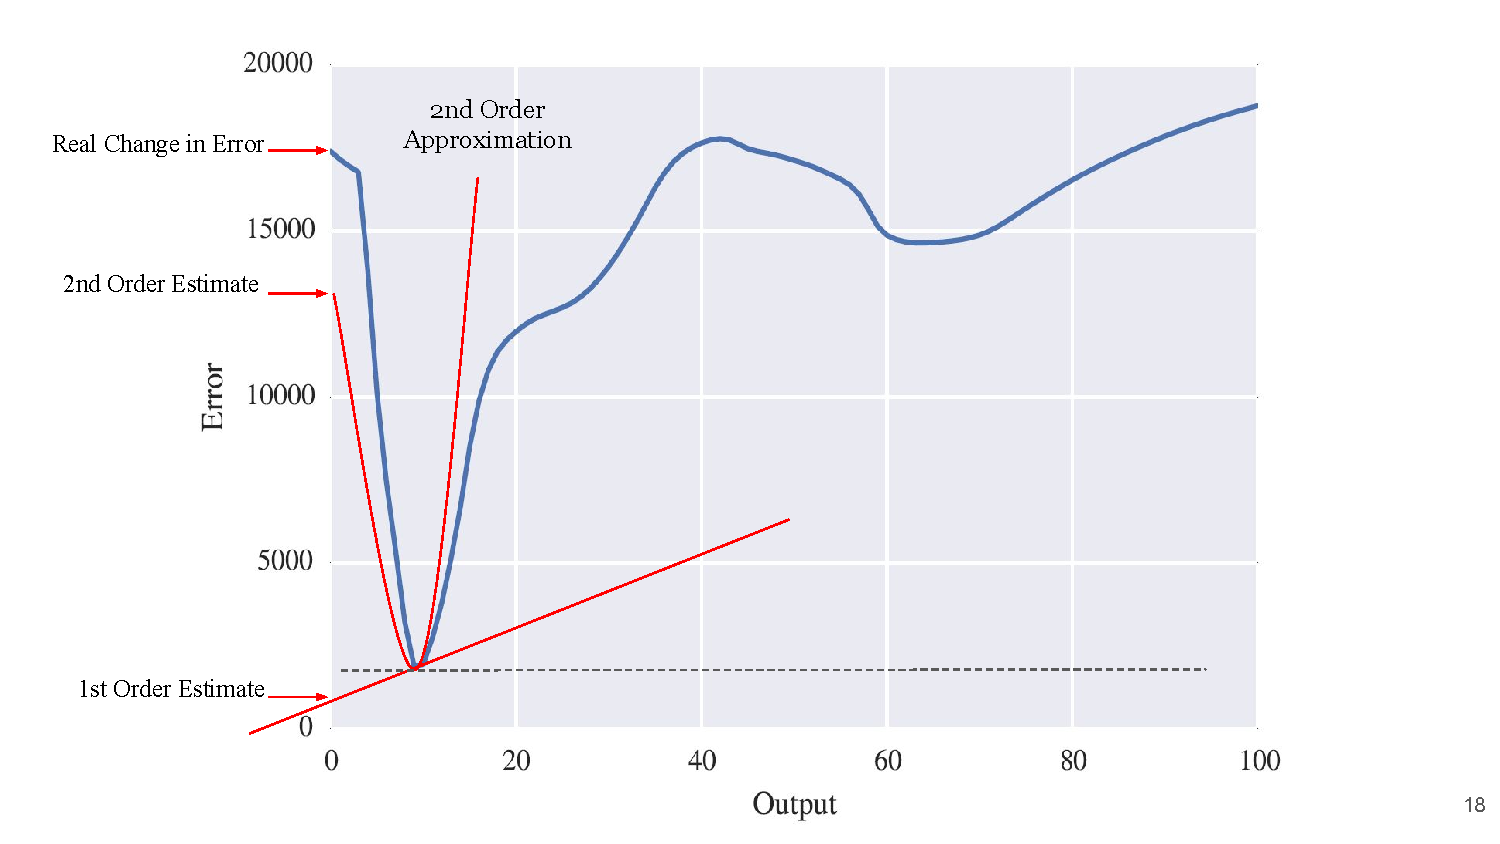
\includegraphics[width=\linewidth]{intuition.pdf}
  \caption{The intuition behind 1st \& 2nd order neuron pruning decisions}
  \label{fig:intuition}
\end{figure}

Figure \ref{fig:intuition} shows a random error function plotted against the output of any given neuron. Note that this figure is for illustration purposes only. The error function is minimized at a particular value of the neuron output as can be seen in the figure. The process of training a neural network is essentially the process of finding these minimizing output values for all the neurons in the network. Pruning this particular neuron (which translates to getting a zero output from it will result in a change in the total overall error. This change in error is represented by distance between the original minimum error (shown by the dashed line) and the top red arrow. This neuron is clearly a bad candidate for removal since removing it will result in a huge error increase. 

The straight red line in the figure represents the first-order approximation of the error using Taylor Series as described before while the parabola represents a second-order approximation. It can be clearly seen that the second-order approximation is a much better estimate of the change in error.

One thing to note here is that it is possible in some cases that there is some thresholding required when trying to approximate the error using the 2nd order Taylor Series expansion. These cases might arise when the parabolic approximation undergoes a steep slope change. To take into account such cases, mean and median thresholding were employed, where any change above a certain threshold was assigned a mean or median value respectively.

Two pruning algorithms are proposed here. They are different in the way the neurons are ranked but both of them use $\Delta E_{k}$, the approximation of the change in error as the basis for the ranking. $\Delta E_{k}$ can be calculated using the Brute Force method, or one of the two Taylor Series approximations discussed previously.

The first step in both the algorithms is to  decide a stopping criterion. This can vary depending on the application but some intuitive stopping criteria can be: maximum number of neurons to remove, percentage scaling needed, maximum allowable accuracy drop etc. 

\subsubsection{Algorithm I: Single Overall Ranking}
The complete algorithm is shown in Algorithm \ref{algo1}. The idea here is to generate a single ranked list based on the values of $\Delta E_{k}$. This involves a single pass of second-order back-propagation (without weight updates) to collect the gradients for each neuron. The neurons from this rank-list (with the lowest values of $\Delta E_{k}$) are then pruned according to the stopping criterion decided. We note here that this algorithm is intentionally naive and is used for comparison only. 

\begin{algorithm}
 \KwData{optimally trained network, training set}
 \KwResult{A pruned network}
 initialize and define stopping criterion \;
 
 perform forward propagation over the training set \;
 
  perform second-order back-propagation without updating weights and collect linear and quadratic gradients \;
  
  rank the remaining neurons based on $\Delta E_{k}$\;
  
 \While{stopping criterion is not met}{
  remove the last ranked neuron \;
  
 }
 \caption{Single Overall Ranking}
 \label{algo1}
\end{algorithm}
 
\subsubsection{Algorithm II: Iterative Re-Ranking}

In this greedy variation of the algorithm (Algorithm \ref{algo2}), after each neuron removal, the remaining network undergoes a single forward and backward pass of second-order back-propagation (without weight updates) and the rank list is formed again. Hence, each removal involves a new pass through the network. This method is computationally more expensive but takes into account the dependencies the neurons might have on one another which would lead to a change in error contribution every time a dependent neuron is removed. 

\begin{algorithm}
 \KwData{optimally trained network, training set}
 \KwResult{A pruned network}
 initialize and define stopping criterion \;
 
 \While{stopping criterion is not met}{
  perform forward propagation over the training set \;
  
  perform second-order back-propagation without updating weights and collect linear and quadratic gradients \;
  
  rank the remaining neurons based on $\Delta E_{k}$  \;
  
  
  remove the worst neuron based on the ranking \;
  
 }
 \caption{Iterative Re-Ranking}
 \label{algo2}
\end{algorithm}
